\section{Can Zooming into Smaller Time Scale Improve Diversity?}
\label{sec:micronano}

% \comment{For micro and nano analysis, on a per rendering
%  interval basis, we scale the rendering interval duration from the power
%  monitor trace to match that of the rendering interval duration of the event
%  trace interval on a per interval basis.}

Performing SPMD by setting up equations at the millisecond scale discussed below
require aligning the power event trace and the power monitor trace at the millisecond scale,
as discussed in \S\ref{subsec:align}.

\subsection{Per-Component SPMD at Micro-Scale}
\label{sec:modelling_micro}

%% 1. Introduction: Zooming into 16.7 ms to extract variation
%%    1a. Explain the variation in 16.7 ms: Busy and idle period
%% 2. Explain how the equations are generated
%% 3. Explain the results
%%    3a. Explain why the solution are not correct
%% 4. Provide the reason for the bad solutions: explain underdetermined equations
%%    4a. Explain 2 variable in GPU
%%    4b. Explain 2 variable in CPU
%%    4c. Explain 4 variable 2 equations
%% 5. Conclusion: Due to underdetermined equations, the solution is infeasible

The repeating app usage across rendering intervals suggests that we
need to zoom into each rendering interval in order to create
multiple equations that are diverse in phone component usage.
Figure~\ref{fig:power_trace_candycrush_menu} shows the power draw
during two 16.7 ms intervals for the Candy Crush Saga Menu scenario.
We observe that there are two distinctive plateaus in each 
16.7 ms interval. The high one is when the GPU is in the Busy state
and the low plateau is when the GPU is in the Idle state.  These two
plateaus provide us with two sub intervals for generating two diverse
equations.  We denote this approach as {\it SPMD at micro-scale}.
\begin{figure*}[tp]
     \centering
     \begin{subfigure}[b]{\textwidth}
         \centering
         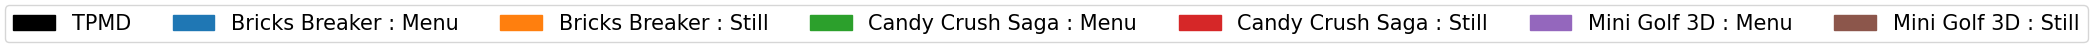
\includegraphics[width=\textwidth]{figures/label_macro_equations.png}
    \end{subfigure}
    \\
    \hfill
    \centering
     \begin{subfigure}[b]{0.31\textwidth}
         \centering
         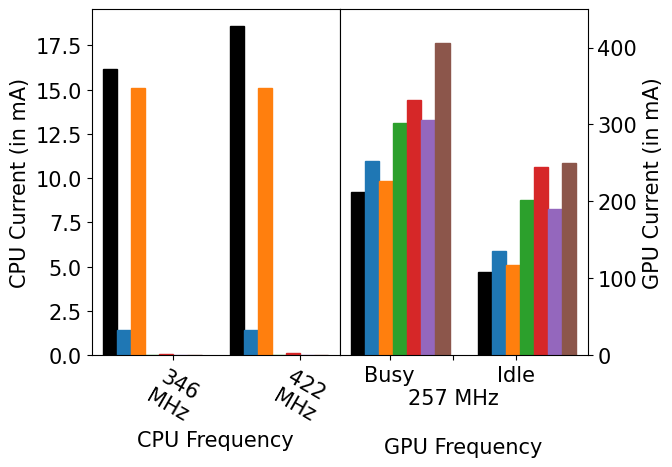
\includegraphics[width=\textwidth]{figures/002_Pixel2_16_micro_equations.png}
         \label{fig:micro_equations_p2}
         \vspace{-0.25in}
         \caption{Pixel 2: TPMD vs micro-SPMD coefficients}
     \end{subfigure}
    \begin{subfigure}[b]{0.32\textwidth}
         \centering
         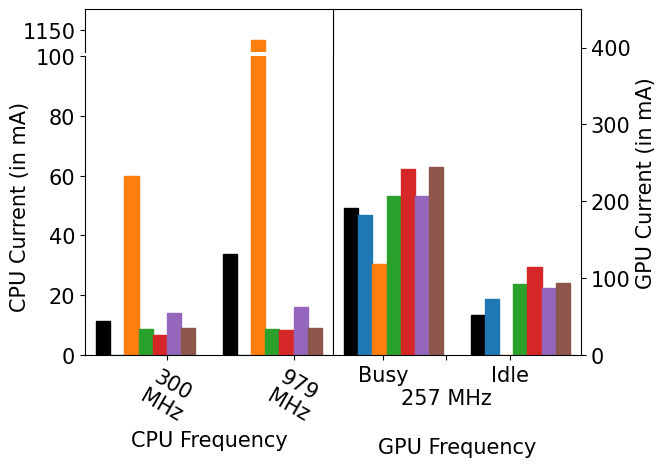
\includegraphics[width=\textwidth]{figures/003_MotoZ3_16_micro_equations.png}
         \label{fig:micro_equations_z3}
         \vspace{-0.25in}
         \caption{Moto Z3: TPMD vs micro-SPMD coefficients}
     \end{subfigure}
    \begin{subfigure}[b]{0.32\textwidth}
         \centering
         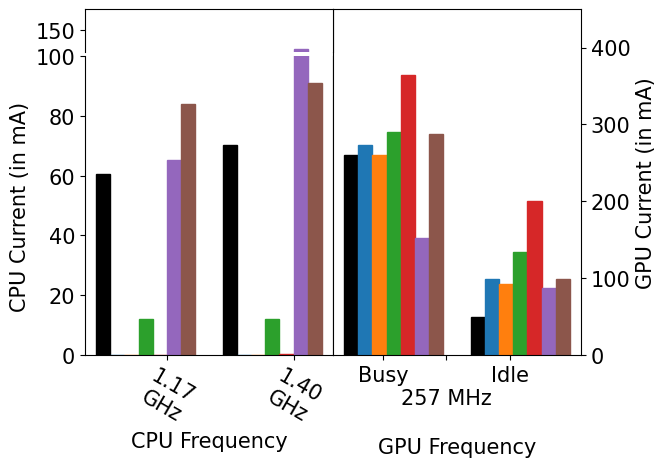
\includegraphics[width=\textwidth]{figures/004_Pixel4_16_micro_equations.png}
         \label{fig:micro_equations_p4}
         \vspace{-0.25in}
         \caption{Pixel 4: TPMD vs micro-SPMD coefficients}
     \end{subfigure}
     \hfill
     \vspace{+0.1in}
     \centering
     \begin{subfigure}[b]{0.31\textwidth}
        \centering
	    \caption{Pixel 2: TPMD vs micro-SPMD error}
	    \vspace{-0.05in}
    	{ \scriptsize
%    	\begin{tabular}{ | p{1.3cm} | p{.2cm} | p{.2cm} | p{.2cm} | p{.2cm} | p{.2cm} | p{.2cm} | }
        \begin{tabular}{ | p{1.8cm} | p{.2cm} | p{.2cm} | p{.2cm} | p{.2cm} | p{.2cm} | p{.2cm} | }
%    	\begin{tabular}{ | l | c | c | c | c | c | c | }
    		\hline
    		     & \multicolumn{6}{ c|}{Error for each App Sc. (\%)}\\
    		\cline{2-7}
                    Model & \rot{B. Menu} & \rot{B. Still} & \rot{C. Menu} & \rot{C. Still} & \rot{M. Menu} & \rot{M. Still}  \\
            \hline
                Fix. F. Const.       & 2.1 & 1.6 & 12 & 13 & 12 & 13 \\
                Classical            & 14 & 25 & 12 & 17 & 13 & 21 \\
            \hline
    	\end{tabular}
    	}
    	% \vspace{-0.05in}
	    % \caption{Pixel 2: TPMD vs micro-SPMD error}
    \end{subfigure}
    \hfill
    \begin{subfigure}[b]{0.31\textwidth}
        \centering
	    \caption{Moto Z3: TPMD vs micro-SPMD error}
	    \vspace{-0.05in}
    	{ \scriptsize
%    	\begin{tabular}{ | p{1.3cm} | p{.2cm} | p{.2cm} | p{.2cm} | p{.2cm} | p{.2cm} | p{.2cm} | }
        \begin{tabular}{ | p{1.8cm} | p{.2cm} | p{.2cm} | p{.2cm} | p{.2cm} | p{.2cm} | p{.2cm} | }
%    	\begin{tabular}{ | l | c | c | c | c | c | c | }
    		\hline
    		     & \multicolumn{6}{ c|}{Error for each App Sc. (\%)}\\
    		\cline{2-7}
                    Model & \rot{B. Menu} & \rot{B. Still} & \rot{C. Menu} & \rot{C. Still} & \rot{M. Menu} & \rot{M. Still}  \\
    		\hline
                Fix. F. Const.       & 7.7 & 16 & 8.5 & 8.1 & 7.4 & 3.6 \\
                Classical            & 30 & 20 & 32 & 19 & 11 & 10 \\
    		\hline
    	\end{tabular}
    	}
    	% \vspace{-0.05in}
	    % \caption{Moto Z3: TPMD vs micro-SPMD error}
    \end{subfigure}
    \hfill
    \begin{subfigure}[b]{0.30\textwidth}
        \centering
	    \caption{Pixel 4: TPMD vs micro-SPMD error}
	    \vspace{-0.05in}
    	{ \scriptsize
%    	\begin{tabular}{ | p{1.3cm} | p{.2cm} | p{.2cm} | p{.2cm} | p{.2cm} | p{.2cm} | p{.2cm} | }
        \begin{tabular}{ | p{1.8cm} | p{.2cm} | p{.2cm} | p{.2cm} | p{.2cm} | p{.2cm} | p{.2cm} | }
%    	\begin{tabular}{ | l | c | c | c | c | c | c | }
    		\hline
    		     & \multicolumn{6}{ c|}{Error for each App Sc. (\%)}\\
    		\cline{2-7}
                    Model & \rot{B. Menu} & \rot{B. Still} & \rot{C. Menu} & \rot{C. Still} & \rot{M. Menu} & \rot{M. Still}  \\
    		\hline
                Fix. F. Const.       & 2.4 & 1.5 & 9.5 & 12 & 3.2 & 6.4 \\
                Classical            & 31 & 35 & 27 & 33 & 20 & 12 \\
    		\hline
    	\end{tabular}
    	}
    	% \vspace{-0.05in}
	    % \caption{Pixel 4: TPMD vs micro-SPMD error}
    \end{subfigure}
    \vspace{-0.1in}
    \caption{Model parameters derived by 8 consecutive 16.7 ms intervals micro-scale SPMD. (Showing the top 2 CPU
        frequencies with high CPU utilization.)(The GPU parameter for TPMD
        is represented by average over all app scenarios GPU parameters.) }
    \label{fig:micro_equations}
    \vspace{-0.1in}
\end{figure*}

\paragraph{Methodology.}
We follow the same methodology as described in
\S\ref{sec:modelling_macro} except that we generated two equations per
16.7 ms interval, one for when GPU is in the Busy state and the other for when 
the GPU is in the Idle
state.
\st{As before, we fixed the base power as a constant to avoid the
under-rank problem and use the Fix. F. Const. % Fix-Freq-Constrained
version of the regression solver.}{\color{blue}--!!-Again, remove and replace Fix. F. Const.  because we no long need the rank -!!--}


% \paragraph{Results.}
% In creating the two equations, we observed that there are more than
% two unknowns as elaborated below.  First, we observe that the GPU almost
% never changes frequency within each 16.7ms interval, and hence it
% contributes two unknowns, \ie for the GPU Busy state and Idle state
% power.  Second, the CPU may change frequency, potentially contributing
% multiple CPU power parameters. This makes the system of two equations
% under-determined. To solve this problem, we tried to set up 2 equations 
% per interval for 4, 8, and 16 intervals, Figure~\ref{fig:micro_equations}
% shows the model parameters output by the regression solver for the six app
% scenarios on the three phones for 8 intervals. 
% The results for other intervals are similar and are omitted due to page limit. 

{\color{blue}We report the modeling results in Figure~\ref{fig:micro_equations}.} We make the following observations.
(1) The power models output by the solver have high LSF{\color{blue}-!!-what is LSF?Maybe it's better not using abbreviation-!!-} error,
between 1.56\%-13.28\% for Pixel 2,
between 3.61\%-15.63\% for Moto Z3,
and between 1.50\%-12.22\% for Pixel 4.
(2) The power parameters range between
0.0$\times$-1.08$\times$,
0.0$\times$-5.75$\times$,
0.0$\times$-1.53$\times$ their
counterparts for CPU frequency for the 3 phones.
(3) The individual power parameters range between
1.14$\times$-1.68$\times$,
0.76$\times$-1.44$\times$,
0.74$\times$-1.42$\times$ their
counterparts for GPU Busy frequency and
1.36$\times$-2.06$\times$,
0.0$\times$-9.48$\times$,
1.22$\times$-28.13$\times$ of their
counterparts for GPU Idle frequency \comment{what is frequency-Idle?? FIXED}
in the TPMD model for Pixel
2, Moto Z3, and Pixel 4, respectively. {\color{blue}We also do the F-test and $R^2$-measurement in Table~?? --EXPLAIN THE TESTING RESULT-- 
As we can see, similar to the situation of macro-scale, at micro-scale SPMD modeling results are still not valid for most of the time. Same explanation in the previous section still applies here, i.e., lack of variation makes the regression result sensitive to the noise.}
\comment{
The high error of these model parameters derived with micro-scale SPMD 
suggests that they cannot capture the power state variation well. 
on what criteria in section 3.6?
}

% \paragraph{Validation.}
% \comment{ 
% How often can we get acceptable solutions for systems of 8 equations? 
% Validation of Micro SPMD using interleaved "training" and "testing" data. 
% Pick 16 equations, form training data using odd equations, and testing data using even equations.
% REMOVING THIS. NOT USED ANYMORE.
% }

\begin{table}[tb]
{\footnotesize
    \centering
    \caption{The 2 smallest singular values for the set of equations for micro-scale "Fix-Freq.-Constr. SPMD" for Pixel 4 for 16 equation system of equation.
    (Top 4 singular values are shown.)
    }
    \vspace{-0.1in}
%    \begin{tabular}{|c|p{9mm}|p{4.5mm}|p{4.5mm}|p{4mm}|p{4mm}|p{4mm}|p{4mm}|c|}
    \begin{tabular}{|c|p{10.5mm}|p{7.5mm}|p{7.5mm}|c|c|c|}
    \hline
        App & Scenario & Num. & Num. &  \multicolumn{2}{c|}{Singular}  & $R^{2}$ \\
            &          &  of &   of &  \multicolumn{2}{c|}{Values}  &   \\
            &          & Eqns. & Vars. &  \multicolumn{2}{c|}{}  & \\
        \hline
         \multirow{2}{13mm}{Bricks Breaker} & Menu & 32 & 6  & 0.17  & 0.12 & 0.99 \\
         \cline{2-7}
         & Still &  32 & 6 & 0.80  & 0.08 & 1.00 \\
         \hline
         \multirow{2}{13mm}{Candy Crush S.} & Menu & 32 & 7 & 0.24  & 0.07 & 0.84 \\
         \cline{2-7}
         & Still & 32 & 7 & 0.17  & 0.04 & 0.65 \\
         \hline
        \multirow{2}{13mm}{Mini Golf 3D} & Menu & 32 & 12 & 0.20  & 0.08 & 0.98 \\
        \cline{2-7}
	     & Still & 32 & 6 & 0.20  & 0.17 & 0.96 \\
	     \hline
    \end{tabular}
    \label{tab:micro_rank_singular}
    \vspace{-0.1in}
}
\end{table}
% \paragraph{Analysis.}
% \comment{
% To understand why some systems can generate reasonable models while
% others cannot, \comment{where do we see this???}
% we plot in Table~\ref{tab:micro_rank_singular} the
% rank and top singular values for the 16-equation systems. 
% We see that all the systems are full rank and have the sufficient number of high
% singular values.
% REMOVING THIS. NOT USED ANYMORE.
% }

\begin{table}[tb]
    \centering
    \caption{Equations for the 8 consecutive 16.7 ms intervals for Bricks Breaker Menu scenario on Moto Z3.}
    {\small
    \vspace{-0.1in}
    \begin{tabular}{|c|c|c|c|c|}
        \hline
             Eqn &    y(n) & \multicolumn{1}{c|}{CPU Utilization} & \multicolumn{2}{c|}{GPU Utilization} \\
        \cline{4-5}
             & (mA) & \multicolumn{1}{c|}{} & Busy & Idle \\
            \hline
               1 & 277.8 & 125\% & 100\% &   0\% \\
               2 & 159.1 & 138\% &   0\% & 100\% \\
               \hline
               3 & 268.6 &  52\% & 100\% &   0\% \\
               4 & 179.3 & 119\% &   3\% &  97\% \\
               \hline
               5 & 318.2 &  69\% & 100\% &   0\% \\
               6 & 160.0 & 132\% &   0\% & 100\% \\
               \hline
               7 & 294.4 &  28\% & 100\% &   0\% \\
               8 & 165.5 & 128\% &   0\% & 100\% \\
               \hline
               9 & 224.9 & 123\% & 100\% &   0\% \\
              10 & 160.3 & 129\% &   0\% & 100\% \\
              \hline
              11 & 293.2 &  50\% & 100\% &   0\% \\
              12 & 168.7 & 130\% &   0\% & 100\% \\
              \hline
              13 & 267.4 &  23\% & 100\% &   0\% \\
              14 & 173.3 & 126\% &   0\% & 100\% \\
              \hline
              15 & 251.5 & 102\% & 100\% &   0\% \\
              16 & 159.8 & 134\% &   0\% & 100\% \\

        \hline
    \end{tabular}
    }
    \label{tab:equations_micro}
    \vspace{-0.1in}
\end{table}

To help readers better understand why SPMD is not able to generate reasonable model,
we take a close look at the system of equations.
% Next,
% we take a close look at two systems, one with acceptable and one
% with unacceptable power parameters generated.
Table~\ref{tab:equations_micro} shows the 16 equations for Bricks
Breaker Menu on Moto Z3
where Equations 1, 3, 5 and 7 correspond to the GPU Busy subintervals
and Equations 2, 4, 6 and 8 correspond to the GPU Idle subintervals
within the rendering intervals.

We make two  observations:
(1) the eight equations for GPU Idle subintervals, 2, 4, 6, 8, 10, 12, 14 and 16, are
very similar in GPU usage and the eight equations for GPU Busy
subintervals, 1, 3, 5, 7, 9, 11, 13, and 15, are very similar in GPU usage.
(2) These two groups differ in CPU utilization which are consistent
with their energy values on the LHS.  We see that the noise in
energy values appear to dominate the diversity in CPU usage.  For
example, the CPU utilization of Eq.~9 and Eq.~11 are 123\% and 50\%,
but their normalized energy value are flipped, at 224.9 mA and 293.2 mA,
respectively.  As a result, the solver is not able to generate
meaningful CPU power parameters.
\comment{ how do we explain the
  energy value variation between Eq.~2 and Eq.~4 does not affect the
  solutions here?  }

\dcomment{
We observe that the $R^2$ value varies between 0.37-0.99, 0.65-0.99 and 0.65-1.00 for the
three phones respectively. This shows that for some app scenarios the
curve\_fit can't fit too well.
For example, for Candy Crush Saga Still on Pixel 4
has a $R^2$ value of 0.65 which is reflected in it's average error of 12\%.
The minimum singular value is 0.04,
causing the system susceptibility to
$0.04^{-1}$$\approx$$25\times$ the measurement noise.
The singular value ratio between the largest and smallest is
4.6$\times$-11.0$\times$, 5.1$\times$-12.1$\times$ and
3.4$\times$-16.6$\times$ on the 3 phones.
The the minimum singular values are between
4.5e-17-0.08,
0.12-0.60
and
0.04-0.17 for the 3 phones respectively.
}

\comment{
These results suggest while zooming into rendering intervals increased the diversity of the systems of equations - they are full rank and have good singular values, but the most of the times the solver cannot output reasonable model parameters due to energy value measurement noise. 
} 

\comment{not sure what to conclude here???}
{\color{blue}Although the modeling results at micro-scale is still not satisfactory for practical use, we do observe better F-test and $R^2$-measurement results that those of the macro-scale.}
